\documentclass[11pt,letterpaper]{article}
\usepackage[utf8]{inputenc}
\usepackage[T1]{fontenc}
\usepackage{lmodern}
\usepackage[spanish,es-nodecimaldot,es-tabla,es-noshorthands]{babel}
\usepackage[top=2.4cm,bottom=2.4cm,left=2.3cm,right=2.3cm]{geometry}
\usepackage{amsmath,amssymb,graphicx,booktabs,longtable,array,float,xcolor,fancyhdr,titlesec,caption,enumitem,microtype,pdflscape,newunicodechar,calc}
\usepackage[hidelinks]{hyperref}
\usepackage{xurl}
\definecolor{azul}{HTML}{164769}
\hypersetup{colorlinks=true,linkcolor=azul,urlcolor=azul,citecolor=azul,pdftitle={CVRP de logística urbana: Etapa 3},pdfauthor={Equipo MA2015}}
\titleformat{\section}{\Large\bfseries\color{azul}}{\thesection.}{0.6em}{}
\titleformat{\subsection}{\large\bfseries\color{azul}}{\thesubsection}{0.6em}{}
\setlength{\parindent}{0pt}\setlength{\parskip}{6pt}
\setlength{\emergencystretch}{2em}
\renewcommand{\arraystretch}{1.15}
\floatplacement{figure}{H}
\setkeys{Gin}{keepaspectratio}
\captionsetup{font=small,labelfont=bf}
\providecommand{\tightlist}{\setlength{\itemsep}{0pt}\setlength{\parskip}{0pt}}
\pagestyle{fancy}\fancyhf{}
\fancyhead[L]{\small Diseño de algoritmos matemáticos bioinspirados}
\fancyhead[R]{\small CVRP $\cdot$ Etapa 3}
\fancyfoot[C]{\thepage}\setlength{\headheight}{14pt}
\renewcommand{\headrulewidth}{0.3pt}
\fancypagestyle{lscape}{\fancyhf{}\fancyfoot[C]{\thepage}\renewcommand{\headrulewidth}{0pt}}
\newunicodechar{±}{\ensuremath{\pm}}
\newunicodechar{²}{\textsuperscript{2}}
\newunicodechar{·}{\ensuremath{\cdot}}
\newunicodechar{×}{\ensuremath{\times}}
\newunicodechar{Σ}{\ensuremath{\Sigma}}
\newunicodechar{α}{\ensuremath{\alpha}}
\newunicodechar{β}{\ensuremath{\beta}}
\newunicodechar{ρ}{\ensuremath{\rho}}
\newunicodechar{τ}{\ensuremath{\tau}}
\newunicodechar{₀}{\textsubscript{0}}
\newunicodechar{→}{\ensuremath{\rightarrow}}
\newunicodechar{∈}{\ensuremath{\in}}
\newunicodechar{−}{\ensuremath{-}}
\newunicodechar{⌈}{\ensuremath{\lceil}}
\newunicodechar{⌉}{\ensuremath{\rceil}}

\begin{document}
\begin{titlepage}
  \centering
  
\includegraphics[width=0.5\textwidth]{figuras/logo_tec.png}\par
  \vspace{2cm}
  {\LARGE\bfseries Entregable 3: comparación de métodos en instancias de referencia\par}
  \vspace{0.5cm}
  {\large Modelo matemático, Clarke--Wright + 2-opt, algoritmo genético y colonia de hormigas para el CVRP\par}
  \vspace{2cm}
  {\large
  Leonardo Orozco -- A00843030\\[2pt]
  Pablo Alonso Robles Nava -- A00573454\\[2pt]
  Sebastián Alberto Chávez Rodríguez -- A01199298\\[2pt]
  Jacqueline Peña San Juan -- A00842524\\[2pt]
  Natalia Ixchel Reynoso Ramírez -- A01352603\par}
  \vspace{1.5cm}
  {\large Profesor: Fernando Elizalde\par}
  \vspace{0.3cm}
  {\large Diseño de algoritmos matemáticos bioinspirados (MA2015) -- Gpo.\ 201\par}
  \vspace{0.3cm}
  {\normalsize Repositorio: \url{https://github.com/Leo-issacs/cvrp-logistica-urbana}\par}
  \vfill
  {\large 26 de octubre de 2026\par}
\end{titlepage}

\begin{abstract}
Se resolvieron 24 instancias de referencia del CVRP (CMT1--CMT14 y diez instancias X de 279 a 458 clientes) con el modelo matemático de la Etapa 1, la heurística propuesta (Clarke--Wright + 2-opt) y los algoritmos genético y de colonia de hormigas de la Etapa 2, con 5 corridas por caso. Contra la mejor solución conocida (BKS), el GAP medio fue de \textbf{7.10 \%} para Clarke--Wright + 2-opt, \textbf{12.41 \%} para la colonia de hormigas y \textbf{18.04 \%} para el algoritmo genético, en sus mejores configuraciones. En el GA la mejor combinación fue \textbf{OX 1 punto, \(p_{m}\) = 0.2, torneo}; en la colonia de hormigas, \textbf{α = 1, β = 5, ρ = 0.1}. Clarke--Wright + 2-opt fue el mejor método en 21 de las 24 instancias y el más rápido: tarda milisegundos, contra segundos de los metaheurísticos. El modelo matemático probó el óptimo solo hasta 30 clientes con un límite de 300 s.
\end{abstract}

\tableofcontents
\newpage

\hypertarget{introducciuxf3n}{%
\section{Introducción}\label{introducciuxf3n}}

Esta etapa cierra el reto del problema de ruteo de vehículos con capacidad (CVRP). En la Etapa 1 se formuló el modelo matemático de arcos y carga (modelo B) y se propuso la heurística de ahorros de Clarke--Wright con mejora 2-opt; en la Etapa 2 se diseñaron un algoritmo genético (GA) y un algoritmo de colonia de hormigas (ACO) sobre una instancia didáctica de 10 clientes. Aquí los cuatro métodos se aplican a 24 instancias de referencia de la literatura, de 50 a 458 clientes, y se responde:

\begin{enumerate}
\def\labelenumi{\arabic{enumi}.}
\tightlist
\item
  ¿Qué nivel de cada hiperparámetro del GA (puntos de cruce, probabilidad de mutación y método de selección) y del ACO (α, β y ρ) da mejores resultados en calidad de la solución, tiempo de cómputo y número de iteraciones?
\item
  ¿Hasta qué tamaño es útil el modelo matemático y qué tan lejos quedan las heurísticas del óptimo que prueba (GAP)?
\item
  ¿Qué algoritmo obtiene los mejores resultados?
\end{enumerate}

\textbf{Nota sobre las instrucciones.} El segundo bloque de combinaciones (α, β y ρ) aparece rotulado como ``Algoritmo Genético'', pero esos son los parámetros del algoritmo de colonia de hormigas; aquí se tratan como tales.

\hypertarget{instancias}{%
\section{Instancias}\label{instancias}}

Se usaron las 24 instancias proporcionadas, en formato TSPLIB de CVRPLIB:

\begin{itemize}
\tightlist
\item
  \textbf{CMT1--CMT14} (Christofides et al., 1979): de 50 a 199 clientes con distancia euclidiana real. Siete de ellas (CMT6--CMT10, CMT13 y CMT14) agregan una \textbf{duración máxima de ruta} D y un \textbf{tiempo de servicio} s por cliente: la suma de distancia recorrida y servicio de cada ruta no puede pasar de D. El objetivo sigue siendo la distancia total.
\item
  \textbf{X-n280 a X-n459} (Uchoa et al., 2017): de 279 a 458 clientes, con distancia euclidiana redondeada al entero más cercano, como en la definición del conjunto.
\end{itemize}

La calidad se mide contra la \textbf{mejor solución conocida (BKS)}: para CMT, el valor que trae cada archivo; para X, el reportado por Vidal (2022).

{\small\setlength{\tabcolsep}{4pt}
\begin{longtable}[]{@{}lrrrrrr@{}}
\caption{Instancias. n = clientes; Q = capacidad; D = duración máxima de ruta; s = tiempo de servicio; \(k_{min}\) = ⌈Σq/Q⌉ (mínimo de vehículos por capacidad).}\tabularnewline
\toprule\noalign{}
Instancia & n & Q & D & s & \(k_{min}\) & BKS \\
\midrule\noalign{}
\endfirsthead
\toprule\noalign{}
Instancia & n & Q & D & s & \(k_{min}\) & BKS \\
\midrule\noalign{}
\endhead
\bottomrule\noalign{}
\endlastfoot
CMT1 & 50 & 160 & --- & --- & 5 & 524.61 \\
CMT2 & 75 & 140 & --- & --- & 10 & 835.26 \\
CMT3 & 100 & 200 & --- & --- & 8 & 826.14 \\
CMT4 & 150 & 200 & --- & --- & 12 & 1,028.42 \\
CMT5 & 199 & 200 & --- & --- & 16 & 1,291.29 \\
CMT6 & 50 & 160 & 200 & 10 & 5 & 555.43 \\
CMT7 & 75 & 140 & 160 & 10 & 10 & 909.68 \\
CMT8 & 100 & 200 & 230 & 10 & 8 & 865.94 \\
CMT9 & 150 & 200 & 200 & 10 & 12 & 1,162.55 \\
CMT10 & 199 & 200 & 200 & 10 & 16 & 1,395.85 \\
CMT11 & 120 & 200 & --- & --- & 7 & 1,042.11 \\
CMT12 & 100 & 200 & --- & --- & 10 & 819.56 \\
CMT13 & 120 & 200 & 720 & 50 & 7 & 1,541.14 \\
CMT14 & 100 & 200 & 1,040 & 90 & 10 & 866.37 \\
X-n280-k17 & 279 & 192 & --- & --- & 17 & 33,503 \\
X-n303-k21 & 302 & 794 & --- & --- & 21 & 21,736 \\
X-n308-k13 & 307 & 246 & --- & --- & 13 & 25,859 \\
X-n327-k20 & 326 & 128 & --- & --- & 20 & 27,532 \\
X-n336-k84 & 335 & 203 & --- & --- & 84 & 139,111 \\
X-n401-k29 & 400 & 745 & --- & --- & 29 & 66,163 \\
X-n411-k19 & 410 & 216 & --- & --- & 19 & 19,712 \\
X-n429-k61 & 428 & 536 & --- & --- & 61 & 65,449 \\
X-n449-k29 & 448 & 777 & --- & --- & 29 & 55,233 \\
X-n459-k26 & 458 & 1106 & --- & --- & 26 & 24,139 \\
\end{longtable}
}

\hypertarget{muxe9todos}{%
\section{Métodos}\label{muxe9todos}}

Los cuatro métodos resuelven el mismo problema: cada cliente se visita exactamente una vez, cada ruta empieza y termina en el depósito, la carga de cada ruta no supera Q y, cuando aplica, la duración de cada ruta no supera D. Toda solución reportada se verificó con una función independiente que revisa estas condiciones y recalcula la distancia.

\hypertarget{modelo-matemuxe1tico-modelo-b-de-la-etapa-1}{%
\subsection{Modelo matemático (modelo B de la Etapa 1)}\label{modelo-matemuxe1tico-modelo-b-de-la-etapa-1}}

Es el modelo de arcos y carga física de la Etapa 1, resuelto con PuLP y CBC. Con \(x_{ij}\) = 1 si un vehículo va de i a j y \(f_{ij}\) = carga que viaja por ese arco:

\[\min \sum_{(i,j)\in A} c_{ij}\,x_{ij}\]

sujeto a

\[\sum_{j\ne i} x_{ji} = 1,\qquad \sum_{j\ne i} x_{ij}=\sum_{j\ne i} x_{ji}\qquad \forall i\in C\]

\[\sum_{j\ne i} f_{ji}-\sum_{j\ne i} f_{ij}=q_i\qquad \forall i\in C\]

\[0\le f_{ij}\le Q\,x_{ij},\qquad \sum_{j\in C} f_{0j}=\sum_{i\in C} q_i,\qquad \sum_{j\in C}x_{0j}\ge k_{\min}\]

donde \(k_{min}\) es el mínimo de vehículos que exige la capacidad (demanda total entre Q, redondeada hacia arriba).

El balance de carga elimina las subrutas sin restricciones explícitas, porque toda demanda es positiva. El modelo tiene n(n+1) variables binarias y otras tantas continuas, así que crece con el cuadrado del número de clientes. No incluye la restricción de duración; por eso el estudio de escalabilidad (sección 8) se hace sobre subinstancias de CMT1, que no la tiene.

\hypertarget{algoritmo-propuesto-clarkewright-2-opt}{%
\subsection{Algoritmo propuesto: Clarke--Wright + 2-opt}\label{algoritmo-propuesto-clarkewright-2-opt}}

Es la heurística propuesta en la Etapa 1, sin cambios de lógica:

\begin{enumerate}
\def\labelenumi{\arabic{enumi}.}
\tightlist
\item
  Cada cliente empieza en su propia ruta 0 → i → 0.
\item
  Se calculan los ahorros \(s_{ij}\) = \(c_{0i}\) + \(c_{0j}\) − \(c_{ij}\) y se ordenan de mayor a menor.
\item
  Se recorren los ahorros: si i y j son extremos de rutas distintas y la ruta unida respeta la capacidad (y la duración, en las instancias que la tienen), se unen.
\item
  Cada ruta final se mejora con 2-opt de mejor mejora hasta que ningún intercambio reduce la distancia.
\end{enumerate}

Para la Etapa 3 solo se agregó la revisión de duración al unir rutas. Es determinista: una sola corrida por instancia; el tiempo reportado es la mediana de 5 ejecuciones.

\hypertarget{algoritmo-genuxe9tico}{%
\subsection{Algoritmo genético}\label{algoritmo-genuxe9tico}}

Se conserva el diseño de la Etapa 2: cada cromosoma es una permutación de los clientes (una ``ruta gigante'') y el decodificador \textbf{Split} (Prins, 2004) la parte de forma óptima en rutas factibles mediante programación dinámica. En esta etapa Split también corta una ruta cuando su duración excede D.

\begin{longtable}[]{@{}
  >{\raggedright\arraybackslash}p{(\columnwidth - 2\tabcolsep) * \real{0.2857}}
  >{\raggedright\arraybackslash}p{(\columnwidth - 2\tabcolsep) * \real{0.7143}}@{}}
\toprule\noalign{}
\begin{minipage}[b]{\linewidth}\raggedright
Elemento
\end{minipage} & \begin{minipage}[b]{\linewidth}\raggedright
Diseño
\end{minipage} \\
\midrule\noalign{}
\endhead
\bottomrule\noalign{}
\endlastfoot
Cromosoma & Permutación de los n clientes \\
Aptitud & Distancia total de la partición óptima que devuelve Split \\
Población & 50 individuos \\
Población inicial & Vecino más cercano aleatorizado: en cada paso se elige al azar uno de los 3 clientes no visitados más cercanos \\
Selección & \textbf{Torneo binario} o \textbf{ruleta} con aptitud 1/costo (factor del experimento) \\
Cruce (\(p_{c}\) = 0.9) & \textbf{OX de un punto} u \textbf{OX de dos puntos} (factor del experimento) \\
Mutación & Inversión de un segmento con probabilidad \textbf{\(p_{m}\) ∈ \{0.1, 0.2, 0.4\}} (factor del experimento) \\
Reemplazo & Elitista: las 2 mejores soluciones de la generación anterior más los 48 mejores hijos \\
Paro & 1,000 generaciones (50,000 soluciones evaluadas) \\
\end{longtable}
\addtocounter{table}{-1}

\textbf{Operadores de cruce.} El OX de dos puntos es el de la Etapa 2: copia del primer padre el segmento entre dos cortes y llena el resto en el orden circular del segundo padre. El OX de un punto copia el prefijo del primer padre hasta un solo corte y completa con los clientes faltantes en el orden en que aparecen en el segundo padre. Ambos producen siempre permutaciones válidas, así que no hace falta reparar.

\textbf{Por qué cambió la población inicial.} En la Etapa 2 la población era aleatoria, lo que funcionó con 10 clientes. Con cientos de clientes una permutación aleatoria está muy lejos de una buena solución, y 50,000 evaluaciones no alcanzan para recuperarse. Para comprobarlo se corrió la configuración exacta de la Etapa 2 (torneo, OX de dos puntos, \(p_{m}\) = 0.2, población aleatoria) en las 24 instancias; el resultado está en la sección 5.3. Sembrar la población con soluciones constructivas es la práctica de Prins (2004) para el GA con Split.

\hypertarget{colonia-de-hormigas}{%
\subsection{Colonia de hormigas}\label{colonia-de-hormigas}}

Se conserva el Ant System de la Etapa 2 (Dorigo et al., 1996): cada hormiga construye una ruta gigante desde el depósito, Split la parte en rutas, y todas las hormigas depositan feromona 1/costo en las adyacencias de su ruta gigante. La probabilidad de ir de i a j es

\[p_{ij}=\frac{\tau_{ij}^{\alpha}\,\eta_{ij}^{\beta}}{\sum_{l\in N_i}\tau_{il}^{\alpha}\,\eta_{il}^{\beta}},\qquad \eta_{ij}=\frac{1}{c_{ij}}\]

y la actualización es \(\tau_{ij}\leftarrow(1-\rho)\,\tau_{ij}+\sum_k 1/L_k\) sobre los arcos usados por cada hormiga k.

\begin{longtable}[]{@{}
  >{\raggedright\arraybackslash}p{(\columnwidth - 2\tabcolsep) * \real{0.3478}}
  >{\raggedright\arraybackslash}p{(\columnwidth - 2\tabcolsep) * \real{0.6522}}@{}}
\toprule\noalign{}
\begin{minipage}[b]{\linewidth}\raggedright
Elemento
\end{minipage} & \begin{minipage}[b]{\linewidth}\raggedright
Diseño
\end{minipage} \\
\midrule\noalign{}
\endhead
\bottomrule\noalign{}
\endlastfoot
Hormigas & 25 \\
Iteraciones & 2,000 (50,000 soluciones evaluadas, igual que el GA) \\
α (peso de la feromona) & \textbf{1 o 2} (factor del experimento) \\
β (peso de la distancia) & \textbf{2 o 5} (factor del experimento) \\
ρ (evaporación) & \textbf{0.1 o 0.5} (factor del experimento) \\
Feromona inicial & τ₀ = m / \(C^{nn}\), con \(C^{nn}\) el costo de la solución del vecino más cercano (Dorigo y Stützle, 2004) \\
Listas de candidatos & Cada hormiga elige entre los 25 clientes no visitados más cercanos; si todos ya fueron visitados, entre todos los restantes \\
\end{longtable}
\addtocounter{table}{-1}

\textbf{Cambios para escalar.} Con 458 clientes, revisar todos los clientes en cada paso cuesta del orden de n² por hormiga; las listas de candidatos reducen ese costo a 25 operaciones por paso sin cambiar la regla de transición. La feromona inicial fija de la Etapa 2 (τ₀ = 0.01) dejaba de tener sentido con costos de decenas de miles: cada depósito 1/L sería de 5 a 1,400 veces menor que τ₀ (1/L va de \(2\times10^{-3}\) en CMT1 a \(7\times10^{-6}\) en X-n336-k84), y la feromona casi no cambiaría. Por eso se usa la regla estándar τ₀ = m / \(C^{nn}\), que pone a τ₀ en la misma escala que los depósitos.

\hypertarget{pulido-con-2-opt}{%
\subsection{Pulido con 2-opt}\label{pulido-con-2-opt}}

Clarke--Wright incluye 2-opt y el GA y el ACO no. Para que la comparación sea justa, a la mejor solución de cada corrida del GA y del ACO también se le aplica el mismo 2-opt dentro de cada ruta, y se reportan ambos valores: el del algoritmo puro y el pulido. Los hiperparámetros se eligen con el valor puro, que es el que depende de ellos.

\hypertarget{diseuxf1o-experimental}{%
\section{Diseño experimental}\label{diseuxf1o-experimental}}

\begin{longtable}[]{@{}
  >{\raggedright\arraybackslash}p{(\columnwidth - 4\tabcolsep) * \real{0.3130}}
  >{\raggedright\arraybackslash}p{(\columnwidth - 4\tabcolsep) * \real{0.3913}}
  >{\raggedright\arraybackslash}p{(\columnwidth - 4\tabcolsep) * \real{0.2957}}@{}}
\toprule\noalign{}
\begin{minipage}[b]{\linewidth}\raggedright
\end{minipage} & \begin{minipage}[b]{\linewidth}\raggedright
Algoritmo genético
\end{minipage} & \begin{minipage}[b]{\linewidth}\raggedright
Colonia de hormigas
\end{minipage} \\
\midrule\noalign{}
\endhead
\bottomrule\noalign{}
\endlastfoot
Factores & Puntos de cruce \{1, 2\} × \(p_{m}\) \{0.1, 0.2, 0.4\} × selección \{torneo, ruleta\} & α \{1, 2\} × β \{2, 5\} × ρ \{0.1, 0.5\} \\
Combinaciones & 12 & 8 \\
Corridas por combinación e instancia & 5 (semillas 0--4) & 5 (semillas 0--4) \\
Total de corridas & 12 × 24 × 5 = 1,440 & 8 × 24 × 5 = 960 \\
Presupuesto por corrida & 50,000 soluciones evaluadas & 50,000 soluciones evaluadas \\
\end{longtable}
\addtocounter{table}{-1}

\textbf{Métricas.}

\begin{itemize}
\tightlist
\item
  \textbf{Calidad:} GAP = 100 · (z − BKS) / BKS, promedio de las 5 corridas.
\item
  \textbf{Tiempo de cómputo:} segundos de pared por corrida, sin contar la lectura de la instancia ni el pulido 2-opt.
\item
  \textbf{Número de iteraciones:} generación (GA) o iteración (ACO) en la que apareció la mejor solución de la corrida. Como el paro es fijo, esta es la medida de qué tan rápido converge cada configuración; una iteración del GA evalúa 50 soluciones y una del ACO 25.
\end{itemize}

\textbf{Cómo se decide el mejor nivel.} Promediar GAP de instancias muy distintas deja que las difíciles dominen; por eso, además del GAP medio, se usa el \textbf{rango medio}: en cada instancia se ordenan las configuraciones de mejor a peor (1 = mejor) y se promedia ese lugar. La significancia se prueba sobre las 24 instancias emparejadas: prueba de Friedman para comparar todas las configuraciones o los tres niveles de \(p_{m}\), y prueba de rangos con signo de Wilcoxon para los factores de dos niveles (Derrac et al., 2011). Se usa α = 0.05.

\textbf{Equipo.} Python 3.13 con NumPy y Numba (núcleos compilados), Intel Xeon a 2.8 GHz, Linux, dos corridas en paralelo. Todos los algoritmos se midieron en el mismo equipo y en las mismas condiciones, así que los tiempos son comparables entre sí, pero no con los de otro equipo.

\hypertarget{resultados-del-algoritmo-genuxe9tico}{%
\section{Resultados del algoritmo genético}\label{resultados-del-algoritmo-genuxe9tico}}

\hypertarget{las-12-combinaciones}{%
\subsection{Las 12 combinaciones}\label{las-12-combinaciones}}

La tabla 2 ordena las combinaciones por rango medio (1 = la mejor en todas las instancias). Las diferencias entre combinaciones son significativas (Friedman, p \textless{} 0.001).

{\small\setlength{\tabcolsep}{4pt}
\begin{longtable}[]{@{}
  >{\raggedleft\arraybackslash}p{(\columnwidth - 14\tabcolsep) * \real{0.1069}}
  >{\raggedright\arraybackslash}p{(\columnwidth - 14\tabcolsep) * \real{0.1258}}
  >{\raggedleft\arraybackslash}p{(\columnwidth - 14\tabcolsep) * \real{0.0881}}
  >{\raggedleft\arraybackslash}p{(\columnwidth - 14\tabcolsep) * \real{0.1132}}
  >{\raggedleft\arraybackslash}p{(\columnwidth - 14\tabcolsep) * \real{0.0755}}
  >{\raggedleft\arraybackslash}p{(\columnwidth - 14\tabcolsep) * \real{0.1824}}
  >{\raggedleft\arraybackslash}p{(\columnwidth - 14\tabcolsep) * \real{0.1069}}
  >{\raggedleft\arraybackslash}p{(\columnwidth - 14\tabcolsep) * \real{0.2013}}@{}}
\caption{Algoritmo genético: promedio sobre las 24 instancias (5 corridas por instancia).}\tabularnewline
\toprule\noalign{}
\begin{minipage}[b]{\linewidth}\raggedleft
\#
\end{minipage} & \begin{minipage}[b]{\linewidth}\raggedright
Configuración
\end{minipage} & \begin{minipage}[b]{\linewidth}\raggedleft
GAP medio (\%)
\end{minipage} & \begin{minipage}[b]{\linewidth}\raggedleft
GAP con 2-opt (\%)
\end{minipage} & \begin{minipage}[b]{\linewidth}\raggedleft
Rango medio
\end{minipage} & \begin{minipage}[b]{\linewidth}\raggedleft
Instancias donde es la mejor
\end{minipage} & \begin{minipage}[b]{\linewidth}\raggedleft
Tiempo medio (s)
\end{minipage} & \begin{minipage}[b]{\linewidth}\raggedleft
Generación de la mejor solución
\end{minipage} \\
\midrule\noalign{}
\endfirsthead
\toprule\noalign{}
\begin{minipage}[b]{\linewidth}\raggedleft
\#
\end{minipage} & \begin{minipage}[b]{\linewidth}\raggedright
Configuración
\end{minipage} & \begin{minipage}[b]{\linewidth}\raggedleft
GAP medio (\%)
\end{minipage} & \begin{minipage}[b]{\linewidth}\raggedleft
GAP con 2-opt (\%)
\end{minipage} & \begin{minipage}[b]{\linewidth}\raggedleft
Rango medio
\end{minipage} & \begin{minipage}[b]{\linewidth}\raggedleft
Instancias donde es la mejor
\end{minipage} & \begin{minipage}[b]{\linewidth}\raggedleft
Tiempo medio (s)
\end{minipage} & \begin{minipage}[b]{\linewidth}\raggedleft
Generación de la mejor solución
\end{minipage} \\
\midrule\noalign{}
\endhead
\bottomrule\noalign{}
\endlastfoot
1 & 1 pto · 0.2 · torneo & 18.04 & 13.74 & 1.62 & 12 & 0.94 & 942 \\
2 & 1 pto · 0.4 · torneo & 18.08 & 13.89 & 1.62 & 11 & 0.99 & 933 \\
3 & 1 pto · 0.1 · torneo & 20.13 & 14.44 & 2.88 & 1 & 0.92 & 937 \\
4 & 2 pto · 0.1 · torneo & 21.86 & 15.48 & 4.08 & 0 & 0.97 & 956 \\
5 & 2 pto · 0.2 · torneo & 23.30 & 16.24 & 4.83 & 0 & 1.02 & 923 \\
6 & 1 pto · 0.1 · ruleta & 26.30 & 17.90 & 6.29 & 0 & 0.98 & 903 \\
7 & 2 pto · 0.4 · torneo & 28.53 & 18.54 & 7.58 & 0 & 1.10 & 898 \\
8 & 1 pto · 0.2 · ruleta & 27.80 & 18.54 & 7.83 & 0 & 1.02 & 897 \\
9 & 1 pto · 0.4 · ruleta & 28.42 & 18.81 & 8.25 & 0 & 1.05 & 884 \\
10 & 2 pto · 0.4 · ruleta & 31.66 & 20.04 & 10.42 & 0 & 1.17 & 801 \\
11 & 2 pto · 0.2 · ruleta & 32.31 & 20.55 & 11.08 & 0 & 1.14 & 743 \\
12 & 2 pto · 0.1 · ruleta & 32.67 & 20.69 & 11.50 & 0 & 1.14 & 670 \\
\end{longtable}
}

\hypertarget{efecto-de-cada-hiperparuxe1metro}{%
\subsection{Efecto de cada hiperparámetro}\label{efecto-de-cada-hiperparuxe1metro}}

\begin{figure}
\centering
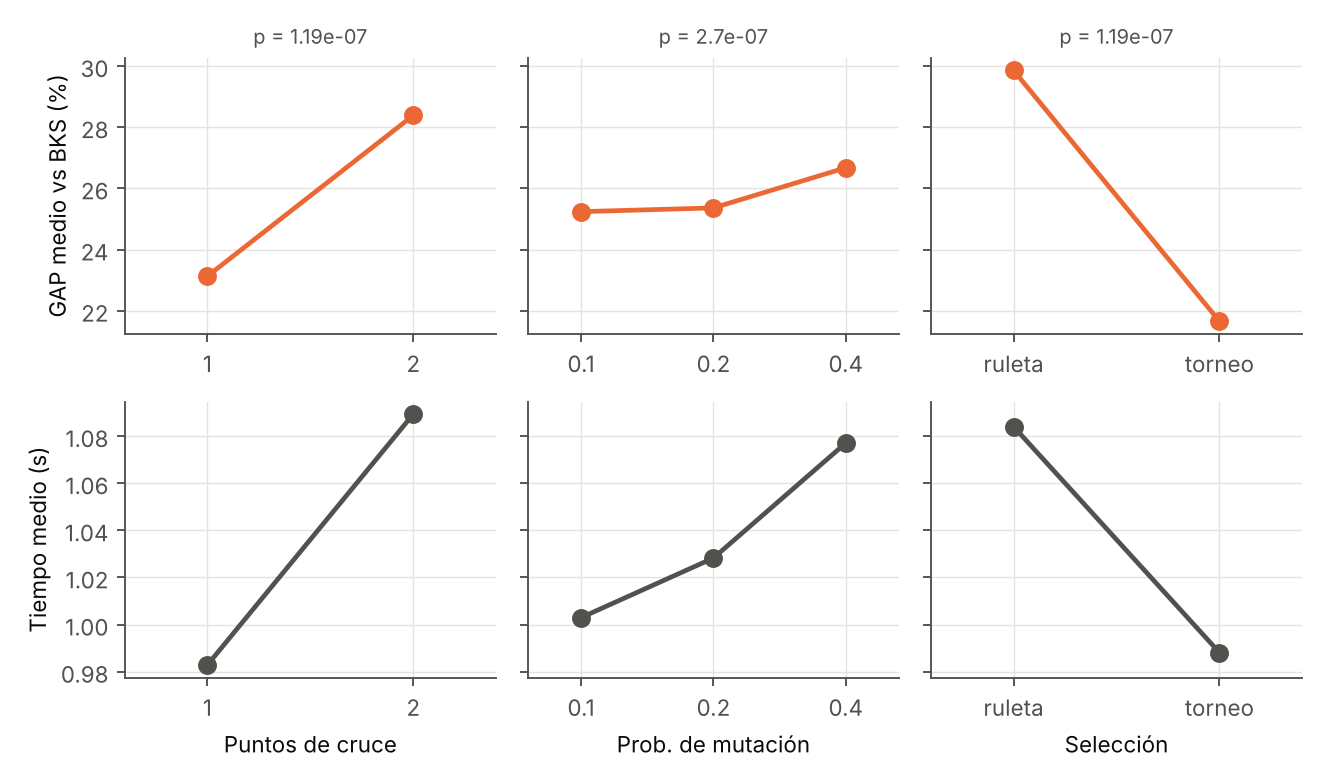
\includegraphics[width=0.95\textwidth,height=\textheight]{figuras/efectos_ga.png}
\caption{Efectos principales del GA: GAP medio (arriba) y tiempo medio (abajo) por nivel. El valor p es el de la prueba sobre las 24 instancias.}
\end{figure}

{\small\setlength{\tabcolsep}{4pt}
\begin{longtable}[]{@{}
  >{\raggedright\arraybackslash}p{(\columnwidth - 10\tabcolsep) * \real{0.1735}}
  >{\raggedright\arraybackslash}p{(\columnwidth - 10\tabcolsep) * \real{0.0612}}
  >{\raggedleft\arraybackslash}p{(\columnwidth - 10\tabcolsep) * \real{0.1429}}
  >{\raggedleft\arraybackslash}p{(\columnwidth - 10\tabcolsep) * \real{0.1224}}
  >{\raggedleft\arraybackslash}p{(\columnwidth - 10\tabcolsep) * \real{0.1735}}
  >{\raggedleft\arraybackslash}p{(\columnwidth - 10\tabcolsep) * \real{0.3265}}@{}}
\caption{Algoritmo genético: promedio por nivel de cada factor (cada nivel promedia todas las combinaciones que lo contienen).}\tabularnewline
\toprule\noalign{}
\begin{minipage}[b]{\linewidth}\raggedright
Factor
\end{minipage} & \begin{minipage}[b]{\linewidth}\raggedright
Nivel
\end{minipage} & \begin{minipage}[b]{\linewidth}\raggedleft
GAP medio (\%)
\end{minipage} & \begin{minipage}[b]{\linewidth}\raggedleft
Rango medio
\end{minipage} & \begin{minipage}[b]{\linewidth}\raggedleft
Tiempo medio (s)
\end{minipage} & \begin{minipage}[b]{\linewidth}\raggedleft
Generación de la mejor solución
\end{minipage} \\
\midrule\noalign{}
\endfirsthead
\toprule\noalign{}
\begin{minipage}[b]{\linewidth}\raggedright
Factor
\end{minipage} & \begin{minipage}[b]{\linewidth}\raggedright
Nivel
\end{minipage} & \begin{minipage}[b]{\linewidth}\raggedleft
GAP medio (\%)
\end{minipage} & \begin{minipage}[b]{\linewidth}\raggedleft
Rango medio
\end{minipage} & \begin{minipage}[b]{\linewidth}\raggedleft
Tiempo medio (s)
\end{minipage} & \begin{minipage}[b]{\linewidth}\raggedleft
Generación de la mejor solución
\end{minipage} \\
\midrule\noalign{}
\endhead
\bottomrule\noalign{}
\endlastfoot
Puntos de cruce & 1 & 23.13 & 4.75 & 0.98 & 916 \\
Puntos de cruce & 2 & 28.39 & 8.25 & 1.09 & 832 \\
Prob. de mutación & 0.1 & 25.24 & 6.19 & 1.00 & 867 \\
Prob. de mutación & 0.2 & 25.36 & 6.34 & 1.03 & 876 \\
Prob. de mutación & 0.4 & 26.67 & 6.97 & 1.08 & 879 \\
Selección & ruleta & 29.86 & 9.23 & 1.08 & 816 \\
Selección & torneo & 21.66 & 3.77 & 0.99 & 932 \\
\end{longtable}
}

\begin{itemize}
\tightlist
\item
  \textbf{Selección.} El torneo binario es mejor que la ruleta en las 24 instancias (GAP medio 21.66 \% contra 29.86 \%; Wilcoxon, p \textless{} 0.001). Con aptitud 1/costo, todas las soluciones de la población tienen costos parecidos, así que la ruleta reparte casi la misma probabilidad a todas y la presión de selección es muy baja. El torneo solo compara dos individuos, sin importar cuánto difieren sus costos. La ruleta también encuentra su mejor solución antes (generación 816 contra 932), pero es porque se estanca, no porque converja mejor.
\item
  \textbf{Puntos de cruce.} El OX de un punto es mejor que el de dos puntos en las 24 instancias (GAP medio 23.13 \% contra 28.39 \%; Wilcoxon, p \textless{} 0.001). El OX de un punto hereda un prefijo completo del primer padre, incluida su conexión con el depósito, y el resto en el orden relativo del segundo, así que conserva bloques largos de rutas ya formadas. El de dos puntos rota el relleno de forma circular y corta más adyacencias. También es un poco más rápido (0.98 s contra 1.09 s).
\item
  \textbf{Probabilidad de mutación.} El efecto es pequeño y depende del cruce. En promedio, \(p_{m}\) = 0.1 y \(p_{m}\) = 0.2 empatan (25.24 \% y 25.36 \%; Wilcoxon, p = 0.439) y ambas son mejores que 0.4 (26.67 \%; p \textless{} 0.001 y p \textless{} 0.001). El mejor nivel cambia según el cruce: con OX de un punto y torneo, 0.2 y 0.4 empatan como los mejores, y con OX de dos puntos y torneo el mejor es 0.1. Un cruce que ya rompe muchas adyacencias necesita menos mutación.
\item
  \textbf{Número de iteraciones.} La mejor combinación encuentra su mejor solución, en promedio, en la generación 942 de 1,000. El GA seguía mejorando al terminar: con más generaciones bajaría más el GAP, y el presupuesto, más que los hiperparámetros, es lo que lo limita.
\end{itemize}

\textbf{Mejor nivel de cada hiperparámetro:} \textbf{OX de un punto, \(p_{m}\) = 0.2 y torneo binario}. Es la combinación con mejor rango medio y la mejor en 12 de las 24 instancias. Empata en rango con \(p_{m}\) = 0.4, pero tiene menor GAP medio y menor tiempo.

\hypertarget{poblaciuxf3n-inicial-aleatoria-etapa-2-contra-heuruxedstica}{%
\subsection{Población inicial: aleatoria (Etapa 2) contra heurística}\label{poblaciuxf3n-inicial-aleatoria-etapa-2-contra-heuruxedstica}}

\begin{longtable}[]{@{}lrrr@{}}
\caption{GA con la configuración de la Etapa 2 (OX de dos puntos, \(p_{m}\) = 0.2, torneo), con población aleatoria y con población heurística. GAP medio de 5 corridas.}\tabularnewline
\toprule\noalign{}
Instancia & n & Población aleatoria (Etapa 2): GAP (\%) & Población heurística: GAP (\%) \\
\midrule\noalign{}
\endfirsthead
\toprule\noalign{}
Instancia & n & Población aleatoria (Etapa 2): GAP (\%) & Población heurística: GAP (\%) \\
\midrule\noalign{}
\endhead
\bottomrule\noalign{}
\endlastfoot
CMT1 & 50 & 14.1 & 10.2 \\
CMT2 & 75 & 23.2 & 14.3 \\
CMT3 & 100 & 54.6 & 22.3 \\
CMT4 & 150 & 94.2 & 31.5 \\
CMT5 & 199 & 116.5 & 32.0 \\
CMT6 & 50 & 15.1 & 10.0 \\
CMT7 & 75 & 29.5 & 17.4 \\
CMT8 & 100 & 57.7 & 24.7 \\
CMT9 & 150 & 86.8 & 36.0 \\
CMT10 & 199 & 119.9 & 37.2 \\
CMT11 & 120 & 73.6 & 14.8 \\
CMT12 & 100 & 48.6 & 11.9 \\
CMT13 & 120 & 56.4 & 13.6 \\
CMT14 & 100 & 53.3 & 13.8 \\
X-n280-k17 & 279 & 142.2 & 29.3 \\
X-n303-k21 & 302 & 146.8 & 29.3 \\
X-n308-k13 & 307 & 192.0 & 38.0 \\
X-n327-k20 & 326 & 173.5 & 31.5 \\
X-n336-k84 & 335 & 39.6 & 13.9 \\
X-n401-k29 & 400 & 99.8 & 14.5 \\
X-n411-k19 & 410 & 225.5 & 38.9 \\
X-n429-k61 & 428 & 102.8 & 18.2 \\
X-n449-k29 & 448 & 163.5 & 23.9 \\
X-n459-k26 & 458 & 200.7 & 31.9 \\
\textbf{Promedio} & & \textbf{97.1} & \textbf{23.3} \\
\end{longtable}

Con población aleatoria el GAP medio es de 97.1 \%, y supera 100 \% en 10 instancias; con la población heurística baja a 23.3 \%. El GA sí aporta sobre su punto de partida: en la mejor configuración, la mejor solución de la población inicial está a 35.52 \% del BKS y la final a 18.04 \%.

\hypertarget{resultados-de-la-colonia-de-hormigas}{%
\section{Resultados de la colonia de hormigas}\label{resultados-de-la-colonia-de-hormigas}}

\hypertarget{las-8-combinaciones}{%
\subsection{Las 8 combinaciones}\label{las-8-combinaciones}}

Las diferencias entre combinaciones son significativas (Friedman, p \textless{} 0.001).

{\small\setlength{\tabcolsep}{4pt}
\begin{longtable}[]{@{}
  >{\raggedleft\arraybackslash}p{(\columnwidth - 14\tabcolsep) * \real{0.1069}}
  >{\raggedright\arraybackslash}p{(\columnwidth - 14\tabcolsep) * \real{0.1321}}
  >{\raggedleft\arraybackslash}p{(\columnwidth - 14\tabcolsep) * \real{0.0881}}
  >{\raggedleft\arraybackslash}p{(\columnwidth - 14\tabcolsep) * \real{0.1132}}
  >{\raggedleft\arraybackslash}p{(\columnwidth - 14\tabcolsep) * \real{0.0755}}
  >{\raggedleft\arraybackslash}p{(\columnwidth - 14\tabcolsep) * \real{0.1824}}
  >{\raggedleft\arraybackslash}p{(\columnwidth - 14\tabcolsep) * \real{0.1069}}
  >{\raggedleft\arraybackslash}p{(\columnwidth - 14\tabcolsep) * \real{0.1950}}@{}}
\caption{Colonia de hormigas: promedio sobre las 24 instancias (5 corridas por instancia).}\tabularnewline
\toprule\noalign{}
\begin{minipage}[b]{\linewidth}\raggedleft
\#
\end{minipage} & \begin{minipage}[b]{\linewidth}\raggedright
Configuración
\end{minipage} & \begin{minipage}[b]{\linewidth}\raggedleft
GAP medio (\%)
\end{minipage} & \begin{minipage}[b]{\linewidth}\raggedleft
GAP con 2-opt (\%)
\end{minipage} & \begin{minipage}[b]{\linewidth}\raggedleft
Rango medio
\end{minipage} & \begin{minipage}[b]{\linewidth}\raggedleft
Instancias donde es la mejor
\end{minipage} & \begin{minipage}[b]{\linewidth}\raggedleft
Tiempo medio (s)
\end{minipage} & \begin{minipage}[b]{\linewidth}\raggedleft
Iteración de la mejor solución
\end{minipage} \\
\midrule\noalign{}
\endfirsthead
\toprule\noalign{}
\begin{minipage}[b]{\linewidth}\raggedleft
\#
\end{minipage} & \begin{minipage}[b]{\linewidth}\raggedright
Configuración
\end{minipage} & \begin{minipage}[b]{\linewidth}\raggedleft
GAP medio (\%)
\end{minipage} & \begin{minipage}[b]{\linewidth}\raggedleft
GAP con 2-opt (\%)
\end{minipage} & \begin{minipage}[b]{\linewidth}\raggedleft
Rango medio
\end{minipage} & \begin{minipage}[b]{\linewidth}\raggedleft
Instancias donde es la mejor
\end{minipage} & \begin{minipage}[b]{\linewidth}\raggedleft
Tiempo medio (s)
\end{minipage} & \begin{minipage}[b]{\linewidth}\raggedleft
Iteración de la mejor solución
\end{minipage} \\
\midrule\noalign{}
\endhead
\bottomrule\noalign{}
\endlastfoot
1 & α = 1, β = 5, ρ = 0.1 & 12.41 & 9.37 & 1.67 & 14 & 2.99 & 815 \\
2 & α = 1, β = 2, ρ = 0.5 & 12.95 & 9.59 & 3.21 & 2 & 2.76 & 738 \\
3 & α = 1, β = 2, ρ = 0.1 & 12.73 & 9.63 & 3.29 & 8 & 3.36 & 1,081 \\
4 & α = 1, β = 5, ρ = 0.5 & 13.23 & 9.88 & 3.62 & 0 & 2.03 & 171 \\
5 & α = 2, β = 2, ρ = 0.1 & 13.65 & 10.17 & 4.62 & 0 & 5.13 & 47 \\
6 & α = 2, β = 5, ρ = 0.1 & 14.09 & 10.49 & 5.21 & 0 & 4.99 & 29 \\
7 & α = 2, β = 2, ρ = 0.5 & 14.59 & 10.87 & 7.04 & 0 & 5.02 & 28 \\
8 & α = 2, β = 5, ρ = 0.5 & 14.87 & 11.05 & 7.33 & 0 & 5.05 & 8 \\
\end{longtable}
}

\hypertarget{efecto-de-cada-hiperparuxe1metro-1}{%
\subsection{Efecto de cada hiperparámetro}\label{efecto-de-cada-hiperparuxe1metro-1}}

\begin{figure}
\centering
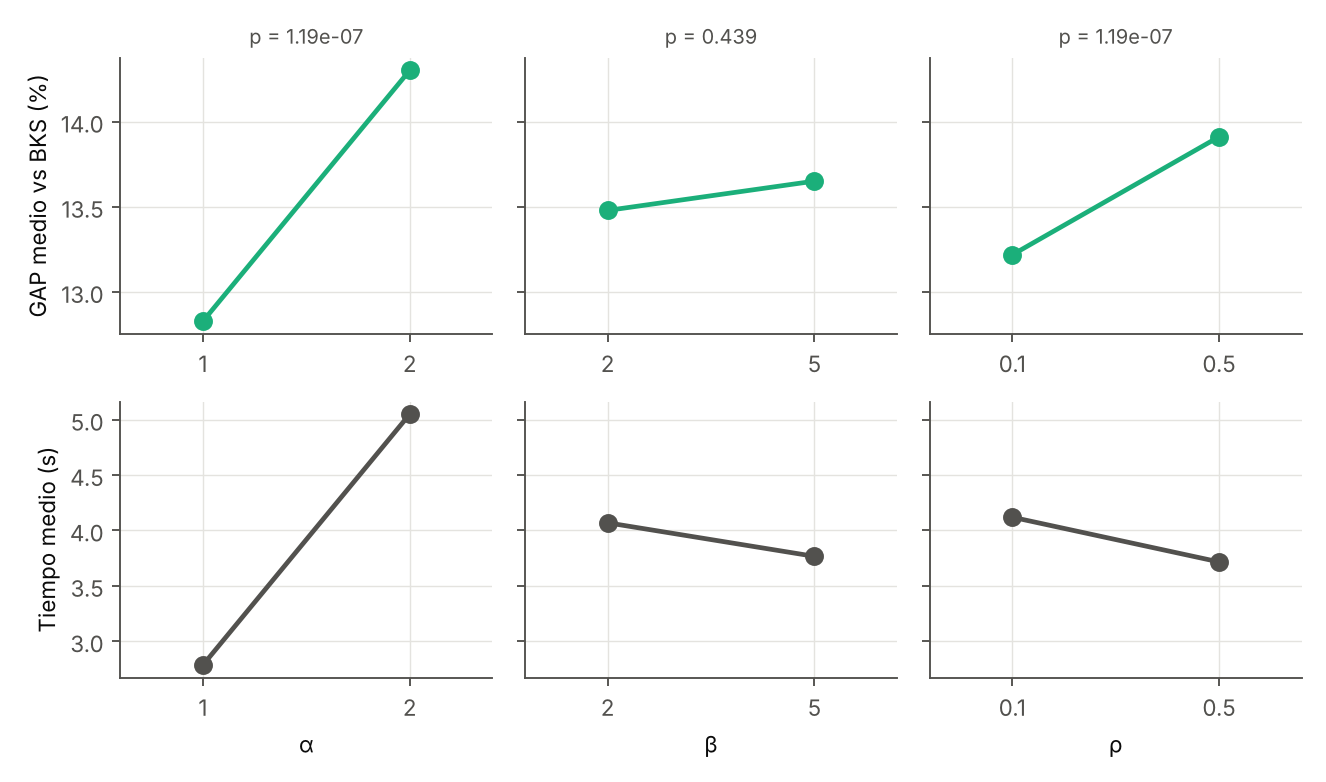
\includegraphics[width=0.95\textwidth,height=\textheight]{figuras/efectos_aco.png}
\caption{Efectos principales del ACO: GAP medio (arriba) y tiempo medio (abajo) por nivel.}
\end{figure}

{\small\setlength{\tabcolsep}{4pt}
\begin{longtable}[]{@{}
  >{\raggedright\arraybackslash}p{(\columnwidth - 10\tabcolsep) * \real{0.1684}}
  >{\raggedright\arraybackslash}p{(\columnwidth - 10\tabcolsep) * \real{0.0526}}
  >{\raggedleft\arraybackslash}p{(\columnwidth - 10\tabcolsep) * \real{0.1474}}
  >{\raggedleft\arraybackslash}p{(\columnwidth - 10\tabcolsep) * \real{0.1263}}
  >{\raggedleft\arraybackslash}p{(\columnwidth - 10\tabcolsep) * \real{0.1789}}
  >{\raggedleft\arraybackslash}p{(\columnwidth - 10\tabcolsep) * \real{0.3263}}@{}}
\caption{Colonia de hormigas: promedio por nivel de cada factor.}\tabularnewline
\toprule\noalign{}
\begin{minipage}[b]{\linewidth}\raggedright
Factor
\end{minipage} & \begin{minipage}[b]{\linewidth}\raggedright
Nivel
\end{minipage} & \begin{minipage}[b]{\linewidth}\raggedleft
GAP medio (\%)
\end{minipage} & \begin{minipage}[b]{\linewidth}\raggedleft
Rango medio
\end{minipage} & \begin{minipage}[b]{\linewidth}\raggedleft
Tiempo medio (s)
\end{minipage} & \begin{minipage}[b]{\linewidth}\raggedleft
Iteración de la mejor solución
\end{minipage} \\
\midrule\noalign{}
\endfirsthead
\toprule\noalign{}
\begin{minipage}[b]{\linewidth}\raggedright
Factor
\end{minipage} & \begin{minipage}[b]{\linewidth}\raggedright
Nivel
\end{minipage} & \begin{minipage}[b]{\linewidth}\raggedleft
GAP medio (\%)
\end{minipage} & \begin{minipage}[b]{\linewidth}\raggedleft
Rango medio
\end{minipage} & \begin{minipage}[b]{\linewidth}\raggedleft
Tiempo medio (s)
\end{minipage} & \begin{minipage}[b]{\linewidth}\raggedleft
Iteración de la mejor solución
\end{minipage} \\
\midrule\noalign{}
\endhead
\bottomrule\noalign{}
\endlastfoot
α & 1 & 12.83 & 2.95 & 2.79 & 701 \\
α & 2 & 14.30 & 6.05 & 5.05 & 28 \\
β & 2 & 13.48 & 4.54 & 4.07 & 474 \\
β & 5 & 13.65 & 4.46 & 3.77 & 256 \\
ρ & 0.1 & 13.22 & 3.70 & 4.12 & 493 \\
ρ & 0.5 & 13.91 & 5.30 & 3.72 & 236 \\
\end{longtable}
}

\begin{itemize}
\tightlist
\item
  \textbf{α (peso de la feromona).} α = 1 es mejor que α = 2 en las 24 instancias (GAP medio 12.83 \% contra 14.30 \%; Wilcoxon, p \textless{} 0.001). Con α = 2 las diferencias de feromona se elevan al cuadrado, la colonia sigue casi siempre los mismos arcos y se estanca: encuentra su mejor solución en la iteración 28 en promedio, contra 701 con α = 1. Además tarda 1.8 veces más, porque cada transición calcula una potencia en vez de usar τ directamente.
\item
  \textbf{ρ (evaporación).} ρ = 0.1 es mejor que ρ = 0.5 en las 24 instancias (13.22 \% contra 13.91 \%; Wilcoxon, p \textless{} 0.001). Con ρ = 0.5 la feromona se olvida en pocas iteraciones, la información se concentra en las últimas soluciones y la búsqueda converge antes (iteración 236 contra 493).
\item
  \textbf{β (peso de la distancia).} En promedio no hay diferencia significativa (13.48 \% con β = 2 y 13.65 \% con β = 5; Wilcoxon, p = 0.439). El efecto depende de los otros dos: β = 5 solo es mejor en la combinación α = 1, ρ = 0.1, que resulta la mejor de todas; en las otras tres combinaciones de α y ρ, β = 2 es ligeramente mejor. Una evaporación lenta mantiene la diversidad que una regla más voraz (β alto) reduciría.
\end{itemize}

\textbf{Mejor nivel de cada hiperparámetro:} \textbf{α = 1, β = 5 y ρ = 0.1}. Es la combinación con mejor rango medio (1.67), la mejor en 14 instancias y la de menor GAP medio (12.41 \%), con un tiempo intermedio. La colonia sí aprende: la mejor solución de la primera iteración está a 22.66 \% del BKS y la final a 12.41 \%.

\hypertarget{comparaciuxf3n-de-los-tres-algoritmos}{%
\section{Comparación de los tres algoritmos}\label{comparaciuxf3n-de-los-tres-algoritmos}}

La tabla 7 compara, instancia por instancia, Clarke--Wright + 2-opt con la mejor configuración del GA y del ACO. GA y ACO son promedios de 5 corridas.

\begin{landscape}
{\footnotesize\setlength{\tabcolsep}{4pt}
\begin{longtable}[]{@{}
  >{\raggedright\arraybackslash}p{(\columnwidth - 22\tabcolsep) * \real{0.1032}}
  >{\raggedleft\arraybackslash}p{(\columnwidth - 22\tabcolsep) * \real{0.0258}}
  >{\raggedleft\arraybackslash}p{(\columnwidth - 22\tabcolsep) * \real{0.0710}}
  >{\raggedleft\arraybackslash}p{(\columnwidth - 22\tabcolsep) * \real{0.0968}}
  >{\raggedleft\arraybackslash}p{(\columnwidth - 22\tabcolsep) * \real{0.0710}}
  >{\raggedleft\arraybackslash}p{(\columnwidth - 22\tabcolsep) * \real{0.0903}}
  >{\raggedleft\arraybackslash}p{(\columnwidth - 22\tabcolsep) * \real{0.0903}}
  >{\raggedleft\arraybackslash}p{(\columnwidth - 22\tabcolsep) * \real{0.0903}}
  >{\raggedleft\arraybackslash}p{(\columnwidth - 22\tabcolsep) * \real{0.0774}}
  >{\raggedleft\arraybackslash}p{(\columnwidth - 22\tabcolsep) * \real{0.0968}}
  >{\raggedleft\arraybackslash}p{(\columnwidth - 22\tabcolsep) * \real{0.0968}}
  >{\raggedleft\arraybackslash}p{(\columnwidth - 22\tabcolsep) * \real{0.0903}}@{}}
\caption{GAP contra el BKS, tiempo y número de iteraciones por instancia.}\tabularnewline
\toprule\noalign{}
\begin{minipage}[b]{\linewidth}\raggedright
Instancia
\end{minipage} & \begin{minipage}[b]{\linewidth}\raggedleft
n
\end{minipage} & \begin{minipage}[b]{\linewidth}\raggedleft
CW GAP (\%)
\end{minipage} & \begin{minipage}[b]{\linewidth}\raggedleft
CW tiempo (ms)
\end{minipage} & \begin{minipage}[b]{\linewidth}\raggedleft
GA GAP (\%)
\end{minipage} & \begin{minipage}[b]{\linewidth}\raggedleft
GA +2-opt (\%)
\end{minipage} & \begin{minipage}[b]{\linewidth}\raggedleft
GA tiempo (s)
\end{minipage} & \begin{minipage}[b]{\linewidth}\raggedleft
GA generación
\end{minipage} & \begin{minipage}[b]{\linewidth}\raggedleft
ACO GAP (\%)
\end{minipage} & \begin{minipage}[b]{\linewidth}\raggedleft
ACO +2-opt (\%)
\end{minipage} & \begin{minipage}[b]{\linewidth}\raggedleft
ACO tiempo (s)
\end{minipage} & \begin{minipage}[b]{\linewidth}\raggedleft
ACO iteración
\end{minipage} \\
\midrule\noalign{}
\endfirsthead
\toprule\noalign{}
\begin{minipage}[b]{\linewidth}\raggedright
Instancia
\end{minipage} & \begin{minipage}[b]{\linewidth}\raggedleft
n
\end{minipage} & \begin{minipage}[b]{\linewidth}\raggedleft
CW GAP (\%)
\end{minipage} & \begin{minipage}[b]{\linewidth}\raggedleft
CW tiempo (ms)
\end{minipage} & \begin{minipage}[b]{\linewidth}\raggedleft
GA GAP (\%)
\end{minipage} & \begin{minipage}[b]{\linewidth}\raggedleft
GA +2-opt (\%)
\end{minipage} & \begin{minipage}[b]{\linewidth}\raggedleft
GA tiempo (s)
\end{minipage} & \begin{minipage}[b]{\linewidth}\raggedleft
GA generación
\end{minipage} & \begin{minipage}[b]{\linewidth}\raggedleft
ACO GAP (\%)
\end{minipage} & \begin{minipage}[b]{\linewidth}\raggedleft
ACO +2-opt (\%)
\end{minipage} & \begin{minipage}[b]{\linewidth}\raggedleft
ACO tiempo (s)
\end{minipage} & \begin{minipage}[b]{\linewidth}\raggedleft
ACO iteración
\end{minipage} \\
\midrule\noalign{}
\endhead
\bottomrule\noalign{}
\endlastfoot
CMT1 & 50 & 11.44 & 1.1 & 10.72 & 10.09 & 0.16 & 713 & 13.43 & 10.14 & 0.33 & 390 \\
CMT2 & 75 & 8.00 & 2.1 & 9.82 & 9.33 & 0.17 & 887 & 9.02 & 7.38 & 0.40 & 355 \\
CMT3 & 100 & 7.00 & 3.5 & 13.72 & 12.20 & 0.36 & 923 & 12.64 & 8.84 & 1.15 & 1,383 \\
CMT4 & 150 & 10.53 & 7.7 & 24.92 & 19.27 & 0.69 & 972 & 13.68 & 10.61 & 1.87 & 1,256 \\
CMT5 & 199 & 7.61 & 13.3 & 26.55 & 20.26 & 0.71 & 979 & 13.82 & 10.81 & 2.63 & 1,202 \\
CMT6 & 50 & 11.34 & 1.0 & 5.10 & 4.77 & 0.13 & 680 & 14.06 & 8.77 & 0.34 & 835 \\
CMT7 & 75 & 7.16 & 2.3 & 12.33 & 12.08 & 0.14 & 975 & 13.31 & 11.71 & 0.36 & 146 \\
CMT8 & 100 & 12.34 & 3.5 & 16.07 & 13.83 & 0.29 & 958 & 16.75 & 14.08 & 1.10 & 1,003 \\
CMT9 & 150 & 10.65 & 8.0 & 25.57 & 23.23 & 0.42 & 954 & 16.03 & 12.37 & 1.63 & 1,053 \\
CMT10 & 199 & 9.53 & 13.6 & 28.46 & 23.89 & 0.62 & 971 & 16.75 & 14.42 & 2.53 & 671 \\
CMT11 & 120 & 0.46 & 4.9 & 6.82 & 3.52 & 0.54 & 976 & 7.42 & 3.35 & 1.07 & 473 \\
CMT12 & 100 & 0.79 & 3.4 & 3.64 & 2.01 & 0.31 & 967 & 3.04 & 1.68 & 0.67 & 114 \\
CMT13 & 120 & 2.91 & 5.2 & 7.60 & 6.09 & 0.38 & 966 & 4.98 & 3.26 & 0.92 & 728 \\
CMT14 & 100 & 0.31 & 3.5 & 5.65 & 3.92 & 0.30 & 949 & 4.45 & 1.85 & 0.64 & 529 \\
X-n280-k17 & 279 & 7.54 & 28.9 & 25.53 & 19.17 & 1.37 & 988 & 15.80 & 11.94 & 4.02 & 914 \\
X-n303-k21 & 302 & 8.76 & 31.0 & 24.97 & 17.77 & 1.48 & 977 & 14.23 & 10.83 & 4.19 & 1,290 \\
X-n308-k13 & 307 & 9.49 & 32.5 & 32.10 & 21.48 & 2.33 & 981 & 18.45 & 14.34 & 5.70 & 981 \\
X-n327-k20 & 326 & 7.93 & 36.2 & 27.79 & 18.51 & 1.48 & 968 & 13.53 & 9.29 & 4.29 & 1,072 \\
X-n336-k84 & 335 & 4.60 & 42.6 & 11.13 & 10.05 & 0.53 & 978 & 11.77 & 11.12 & 3.70 & 718 \\
X-n401-k29 & 400 & 4.15 & 88.7 & 13.09 & 9.42 & 1.92 & 974 & 8.43 & 6.44 & 6.34 & 589 \\
X-n411-k19 & 410 & 8.63 & 65.1 & 33.69 & 21.68 & 2.88 & 979 & 20.21 & 14.79 & 7.73 & 1,300 \\
X-n429-k61 & 428 & 4.66 & 86.4 & 16.38 & 12.35 & 0.90 & 994 & 9.39 & 7.33 & 5.11 & 309 \\
X-n449-k29 & 448 & 5.80 & 90.7 & 22.05 & 14.83 & 1.94 & 955 & 12.59 & 9.20 & 7.27 & 1,485 \\
X-n459-k26 & 458 & 8.87 & 91.4 & 29.27 & 20.04 & 2.39 & 940 & 13.96 & 10.42 & 7.73 & 772 \\
\textbf{Promedio} & & \textbf{7.10} & 27.8 & \textbf{18.04} & 13.74 & 0.94 & 942 & \textbf{12.41} & 9.37 & 2.99 & 815 \\
\end{longtable}
}
\end{landscape}

\begin{figure}
\centering
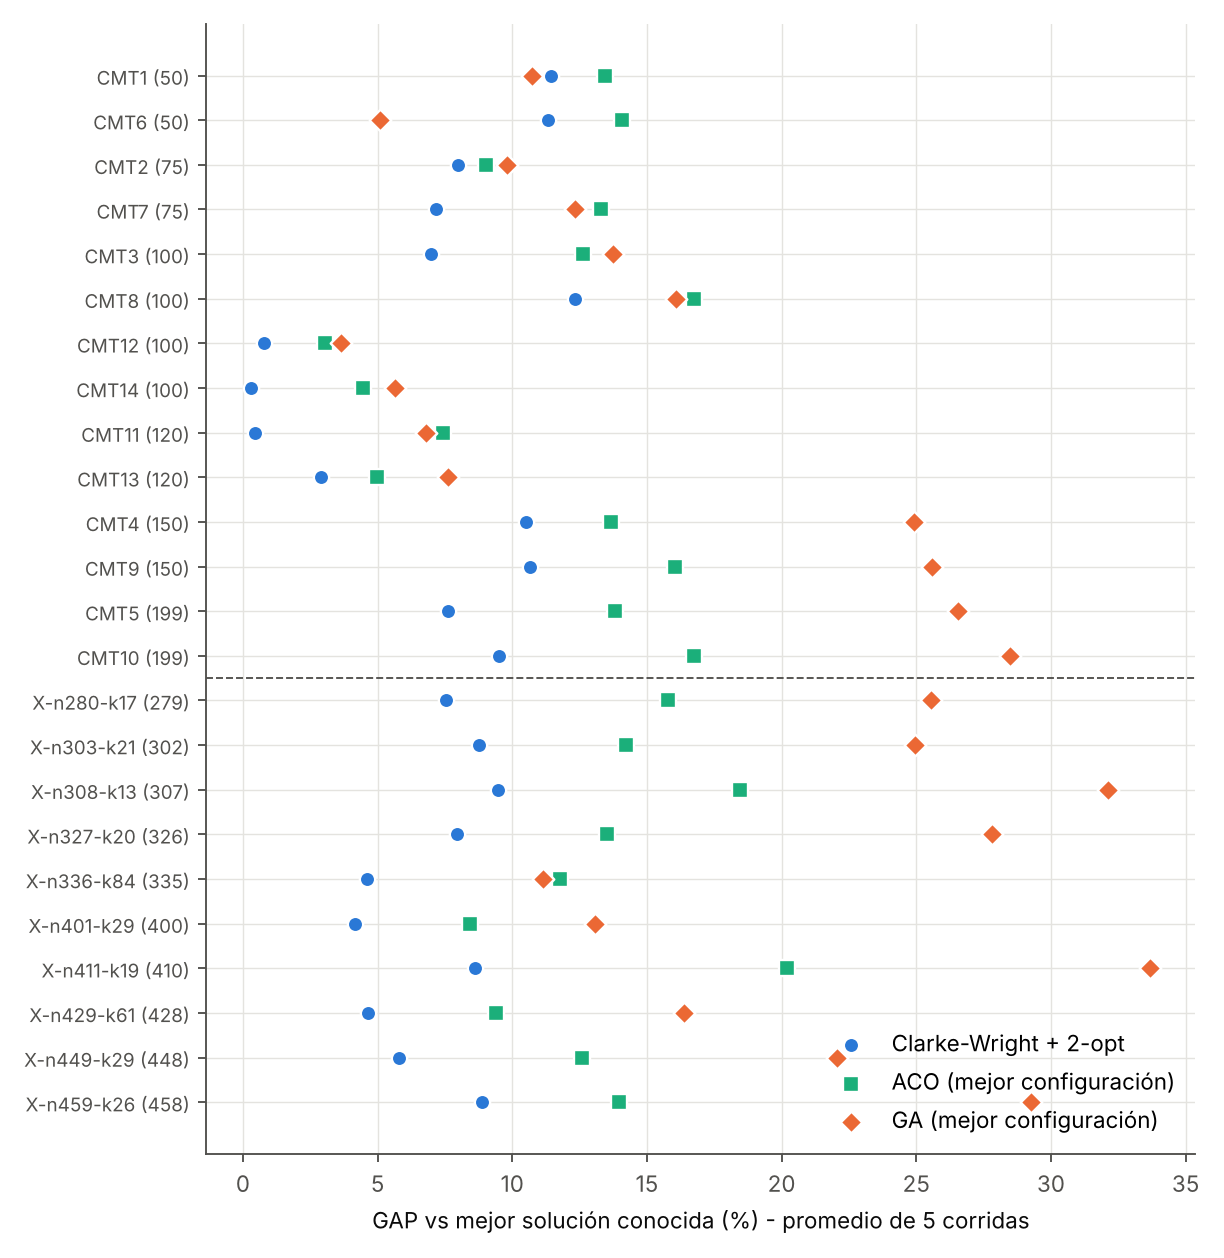
\includegraphics[width=0.85\textwidth,height=\textheight]{figuras/comparacion_gap.png}
\caption{GAP de cada método por instancia (las instancias X están debajo de la línea punteada).}
\end{figure}

\textbf{Calidad de la solución.} Clarke--Wright + 2-opt tiene el menor GAP medio (7.10 \%), seguido del ACO (12.41 \%; 9.37 \% con 2-opt) y del GA (18.04 \%; 13.74 \% con 2-opt). Aun con el mismo 2-opt aplicado a sus soluciones, CW es el mejor en 21 instancias; el GA gana en 2 (CMT1, CMT6) y el ACO en 1 (CMT2). La ventaja de CW crece con el tamaño: en las instancias X su GAP medio es 7.04 \%, contra 13.84 \% del ACO y 23.60 \% del GA. Las instancias agrupadas (CMT11--CMT14) son las más fáciles para todos.

\textbf{Tiempo de cómputo.} CW + 2-opt tarda de 1.0 a 91.4 ms por instancia. El GA tarda 0.94 s en promedio y el ACO 2.99 s, con el mismo número de soluciones evaluadas: construir una solución con hormigas cuesta más que cruzar dos permutaciones.

\begin{figure}
\centering
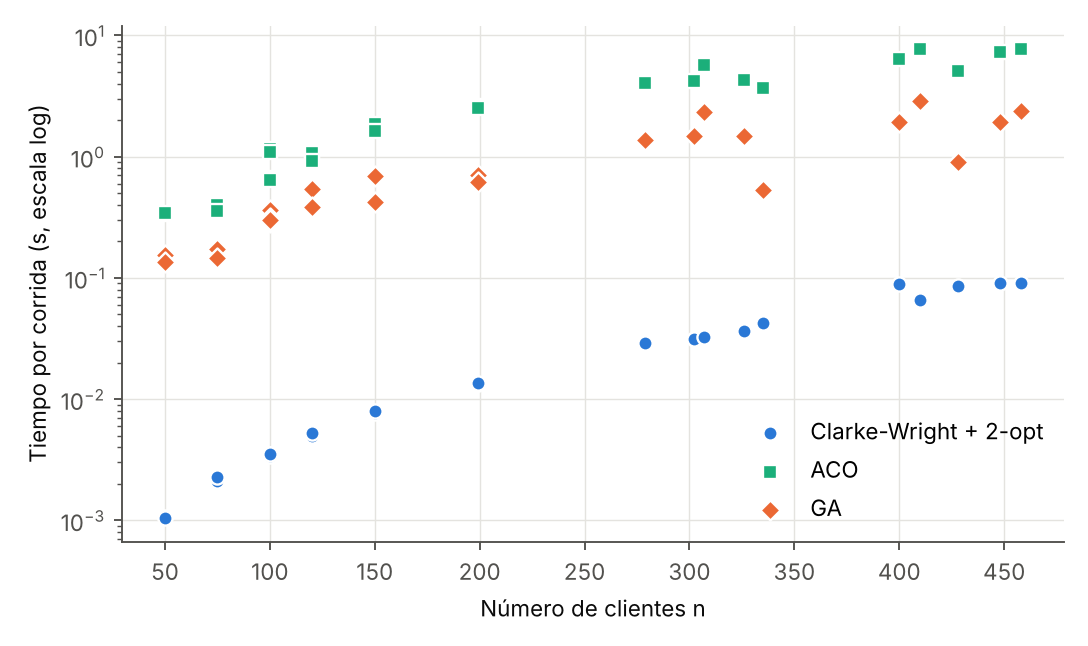
\includegraphics[width=0.8\textwidth,height=\textheight]{figuras/tiempos.png}
\caption{Tiempo por corrida contra número de clientes.}
\end{figure}

\textbf{Número de iteraciones.} El GA encuentra su mejor solución cerca del final (generación 942 de 1,000 en promedio) y el ACO a la mitad (iteración 815 de 2,000). En la figura de convergencia, el GA sigue bajando al terminar, mientras que la colonia se aplana: el GA está limitado por el presupuesto y el ACO por su propia convergencia. CW no itera: construye su solución en una sola pasada.

\begin{figure}
\centering
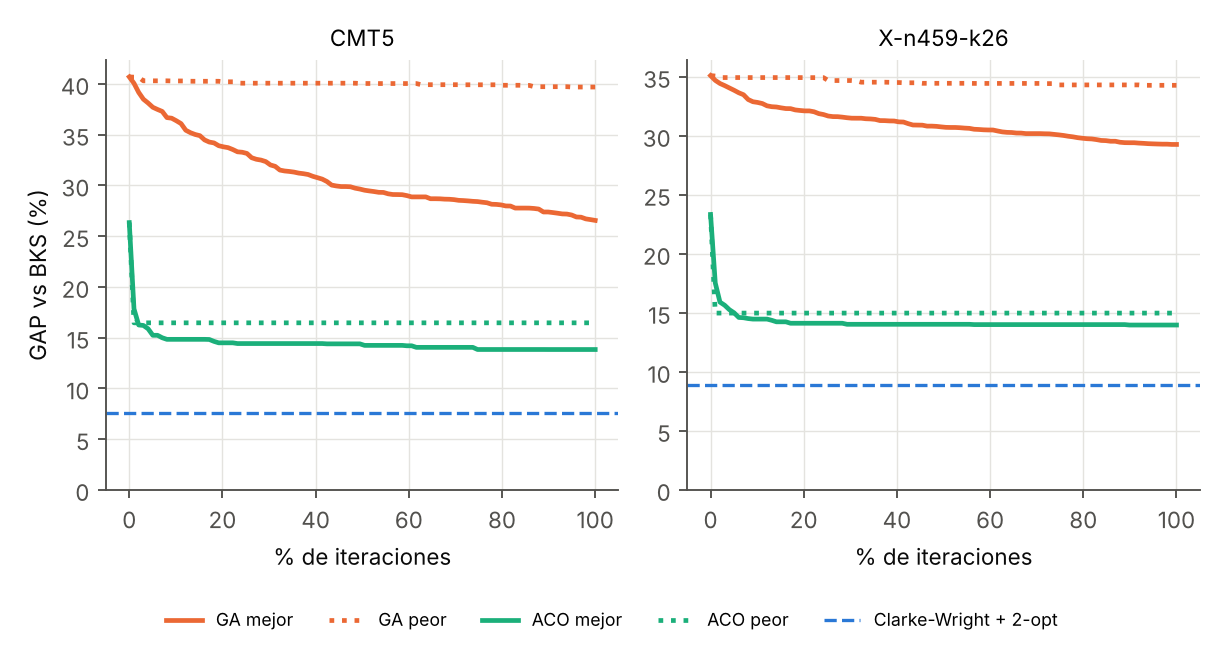
\includegraphics[width=0.95\textwidth,height=\textheight]{figuras/convergencia.png}
\caption{Convergencia media (5 corridas) de la mejor y la peor configuración de cada algoritmo, en CMT5 y X-n459-k26. La línea discontinua es Clarke--Wright + 2-opt.}
\end{figure}

\hypertarget{comparaciuxf3n-con-el-modelo-matemuxe1tico}{%
\section{Comparación con el modelo matemático}\label{comparaciuxf3n-con-el-modelo-matemuxe1tico}}

El modelo matemático da el óptimo, pero no escala. Se resolvió con CBC (límite de 300 s por corrida) en subinstancias de CMT1 con el depósito y los primeros k clientes, y en CMT1 completa. En cada subinstancia se corrieron también CW + 2-opt y la mejor configuración del GA y del ACO (5 corridas). El GAP de esta tabla se mide contra el \textbf{óptimo probado por el modelo}, no contra el BKS.

\begin{landscape}
{\footnotesize\setlength{\tabcolsep}{4pt}
\begin{longtable}[]{@{}
  >{\raggedleft\arraybackslash}p{(\columnwidth - 18\tabcolsep) * \real{0.1090}}
  >{\raggedleft\arraybackslash}p{(\columnwidth - 18\tabcolsep) * \real{0.0641}}
  >{\raggedleft\arraybackslash}p{(\columnwidth - 18\tabcolsep) * \real{0.0897}}
  >{\raggedright\arraybackslash}p{(\columnwidth - 18\tabcolsep) * \real{0.1282}}
  >{\raggedleft\arraybackslash}p{(\columnwidth - 18\tabcolsep) * \real{0.1346}}
  >{\raggedleft\arraybackslash}p{(\columnwidth - 18\tabcolsep) * \real{0.1154}}
  >{\raggedleft\arraybackslash}p{(\columnwidth - 18\tabcolsep) * \real{0.1410}}
  >{\raggedleft\arraybackslash}p{(\columnwidth - 18\tabcolsep) * \real{0.0705}}
  >{\raggedleft\arraybackslash}p{(\columnwidth - 18\tabcolsep) * \real{0.0705}}
  >{\raggedleft\arraybackslash}p{(\columnwidth - 18\tabcolsep) * \real{0.0769}}@{}}
\caption{Escalabilidad del modelo y GAP de los algoritmos contra el óptimo.}\tabularnewline
\toprule\noalign{}
\begin{minipage}[b]{\linewidth}\raggedleft
Clientes
\end{minipage} & \begin{minipage}[b]{\linewidth}\raggedleft
Variables
\end{minipage} & \begin{minipage}[b]{\linewidth}\raggedleft
Restricciones
\end{minipage} & \begin{minipage}[b]{\linewidth}\raggedright
Estado de CBC
\end{minipage} & \begin{minipage}[b]{\linewidth}\raggedleft
Distancia del modelo
\end{minipage} & \begin{minipage}[b]{\linewidth}\raggedleft
Brecha de CBC (\%)
\end{minipage} & \begin{minipage}[b]{\linewidth}\raggedleft
Tiempo del modelo (s)
\end{minipage} & \begin{minipage}[b]{\linewidth}\raggedleft
GAP CW (\%)
\end{minipage} & \begin{minipage}[b]{\linewidth}\raggedleft
GAP GA (\%)
\end{minipage} & \begin{minipage}[b]{\linewidth}\raggedleft
GAP ACO (\%)
\end{minipage} \\
\midrule\noalign{}
\endfirsthead
\toprule\noalign{}
\begin{minipage}[b]{\linewidth}\raggedleft
Clientes
\end{minipage} & \begin{minipage}[b]{\linewidth}\raggedleft
Variables
\end{minipage} & \begin{minipage}[b]{\linewidth}\raggedleft
Restricciones
\end{minipage} & \begin{minipage}[b]{\linewidth}\raggedright
Estado de CBC
\end{minipage} & \begin{minipage}[b]{\linewidth}\raggedleft
Distancia del modelo
\end{minipage} & \begin{minipage}[b]{\linewidth}\raggedleft
Brecha de CBC (\%)
\end{minipage} & \begin{minipage}[b]{\linewidth}\raggedleft
Tiempo del modelo (s)
\end{minipage} & \begin{minipage}[b]{\linewidth}\raggedleft
GAP CW (\%)
\end{minipage} & \begin{minipage}[b]{\linewidth}\raggedleft
GAP GA (\%)
\end{minipage} & \begin{minipage}[b]{\linewidth}\raggedleft
GAP ACO (\%)
\end{minipage} \\
\midrule\noalign{}
\endhead
\bottomrule\noalign{}
\endlastfoot
5 & 60 & 54 & Óptimo probado & 107.02 & 0.00 & 0.0 & 0.00 & 0.00 & 0.00 \\
8 & 144 & 108 & Óptimo probado & 146.72 & 0.00 & 0.1 & 1.38 & 0.83 & 0.00 \\
10 & 220 & 154 & Óptimo probado & 168.23 & 0.00 & 0.1 & 5.63 & 0.00 & 0.00 \\
12 & 312 & 208 & Óptimo probado & 194.64 & 0.00 & 0.7 & 7.16 & 1.36 & 2.78 \\
15 & 480 & 304 & Óptimo probado & 238.67 & 0.00 & 0.9 & 7.01 & 1.89 & 0.35 \\
20 & 840 & 504 & Óptimo probado & 291.24 & 0.00 & 3.8 & 3.59 & 1.61 & 3.90 \\
25 & 1,300 & 754 & Óptimo probado & 327.94 & 0.00 & 37.7 & 5.74 & 4.44 & 4.97 \\
30 & 1,860 & 1,054 & Óptimo probado & 358.46 & 0.00 & 12.9 & 7.25 & 7.16 & 4.43 \\
35 & 2,520 & 1,404 & Factible, sin prueba & 404.87 & 1.90 & 300.9 & --- & --- & --- \\
40 & 3,280 & 1,804 & Factible, sin prueba & 519.56 & 16.32 & 300.3 & --- & --- & --- \\
45 & 4,140 & 2,254 & Factible, sin prueba & 541.05 & 10.16 & 300.3 & --- & --- & --- \\
50 & 5,100 & 2,754 & Factible, sin prueba & 562.96 & 10.31 & 300.4 & --- & --- & --- \\
\end{longtable}
}
\end{landscape}

\begin{figure}
\centering
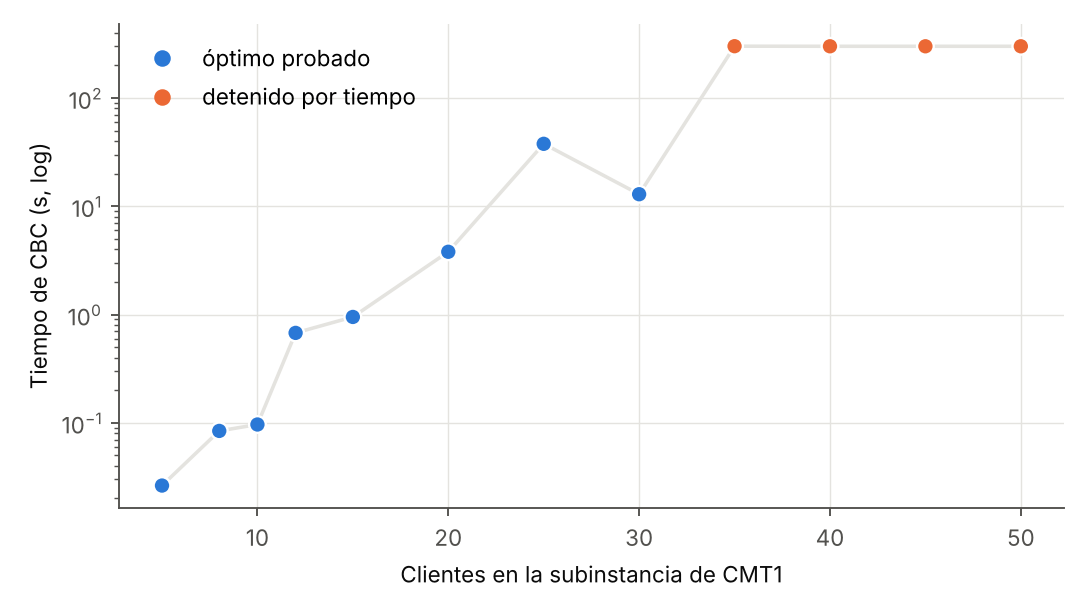
\includegraphics[width=0.8\textwidth,height=\textheight]{figuras/escalabilidad_modelo.png}
\caption{Tiempo de CBC contra número de clientes.}
\end{figure}

\textbf{Hasta dónde escala.} CBC probó el óptimo en todas las subinstancias de hasta 30 clientes. El tiempo creció de 0.03 s con 5 clientes a 37.7 s con 25; no crece de forma monótona porque depende de qué tan rápido la ramificación y acotamiento cierra la brecha. Con 35 clientes se detuvo a los 300 s con una solución de 404.87 (mejor que la de CW, 451.13) y una cota inferior de 397.20: brecha de 1.90 \%. Con 40 clientes se detuvo a los 300 s con una solución de 519.56 (peor que la de CW, 496.32) y una cota inferior de 434.75: brecha de 16.32 \%. Con 45 clientes se detuvo a los 300 s con una solución de 541.05 (mejor que la de CW, 563.71) y una cota inferior de 486.05: brecha de 10.16 \%. Con 50 clientes se detuvo a los 300 s con una solución de 562.96 (mejor que la de CW, 584.64) y una cota inferior de 504.93: brecha de 10.31 \%. El número de variables crece con el cuadrado de n: una instancia X de 458 clientes tendría unas 420,000 variables, la mitad binarias, así que el modelo no es aplicable en ese tamaño.

\textbf{GAP contra el óptimo.} En las 8 subinstancias con óptimo probado, el GAP medio fue de 4.72 \% para CW + 2-opt, 2.16 \% para el GA y 2.05 \% para el ACO (promedios de 5 corridas). En estos tamaños pequeños el orden se invierte respecto de las instancias grandes: los dos metaheurísticos superan a CW, y la mejor de sus 5 corridas alcanzó el óptimo en 5 subinstancias (GA) y 4 (ACO). Con pocos clientes, 50,000 evaluaciones bastan para explorar bien el espacio; con cientos, no.

En CMT1 completa, la solución que CBC tenía a los 300 s (562.96) fue mejor que la de CW (584.64), el GA (580.87) y el ACO (595.08), pero sigue 7.31 \% arriba del BKS (524.61) y no trae garantía de optimalidad. Con 40 clientes pasó lo contrario: la solución del solver fue peor que la de CW. Detenido por tiempo, el modelo es una heurística más, sin certeza de su calidad.

\hypertarget{corrida-final-con-los-mejores-hiperparuxe1metros}{%
\section{Corrida final con los mejores hiperparámetros}\label{corrida-final-con-los-mejores-hiperparuxe1metros}}

Para confirmar la elección se corrieron de nuevo el GA (OX 1 punto, \(p_{m}\) = 0.2, torneo) y el ACO (α = 1, β = 5, ρ = 0.1) en las 24 instancias con 5 semillas nuevas (5 a 9), que no se usaron para elegir los hiperparámetros.

{\small\setlength{\tabcolsep}{4pt}
\begin{longtable}[]{@{}
  >{\raggedright\arraybackslash}p{(\columnwidth - 12\tabcolsep) * \real{0.1333}}
  >{\raggedleft\arraybackslash}p{(\columnwidth - 12\tabcolsep) * \real{0.1583}}
  >{\raggedleft\arraybackslash}p{(\columnwidth - 12\tabcolsep) * \real{0.1500}}
  >{\raggedleft\arraybackslash}p{(\columnwidth - 12\tabcolsep) * \real{0.1250}}
  >{\raggedleft\arraybackslash}p{(\columnwidth - 12\tabcolsep) * \real{0.1583}}
  >{\raggedleft\arraybackslash}p{(\columnwidth - 12\tabcolsep) * \real{0.1333}}
  >{\raggedright\arraybackslash}p{(\columnwidth - 12\tabcolsep) * \real{0.1417}}@{}}
\caption{Corrida final: GAP medio de 5 corridas nuevas.}\tabularnewline
\toprule\noalign{}
\begin{minipage}[b]{\linewidth}\raggedright
Instancia
\end{minipage} & \begin{minipage}[b]{\linewidth}\raggedleft
CW + 2-opt GAP (\%)
\end{minipage} & \begin{minipage}[b]{\linewidth}\raggedleft
GA GAP (\%) ± d.e.
\end{minipage} & \begin{minipage}[b]{\linewidth}\raggedleft
GA + 2-opt (\%)
\end{minipage} & \begin{minipage}[b]{\linewidth}\raggedleft
ACO GAP (\%) ± d.e.
\end{minipage} & \begin{minipage}[b]{\linewidth}\raggedleft
ACO + 2-opt (\%)
\end{minipage} & \begin{minipage}[b]{\linewidth}\raggedright
Mejor (con 2-opt)
\end{minipage} \\
\midrule\noalign{}
\endfirsthead
\toprule\noalign{}
\begin{minipage}[b]{\linewidth}\raggedright
Instancia
\end{minipage} & \begin{minipage}[b]{\linewidth}\raggedleft
CW + 2-opt GAP (\%)
\end{minipage} & \begin{minipage}[b]{\linewidth}\raggedleft
GA GAP (\%) ± d.e.
\end{minipage} & \begin{minipage}[b]{\linewidth}\raggedleft
GA + 2-opt (\%)
\end{minipage} & \begin{minipage}[b]{\linewidth}\raggedleft
ACO GAP (\%) ± d.e.
\end{minipage} & \begin{minipage}[b]{\linewidth}\raggedleft
ACO + 2-opt (\%)
\end{minipage} & \begin{minipage}[b]{\linewidth}\raggedright
Mejor (con 2-opt)
\end{minipage} \\
\midrule\noalign{}
\endhead
\bottomrule\noalign{}
\endlastfoot
CMT1 & 11.44 & 9.59 ± 3.75 & 9.59 & 12.58 ± 2.97 & 8.93 & ACO \\
CMT2 & 8.00 & 9.93 ± 1.98 & 9.59 & 8.92 ± 0.55 & 7.40 & ACO \\
CMT3 & 7.00 & 15.71 ± 3.49 & 12.99 & 11.82 ± 0.82 & 9.29 & CW \\
CMT4 & 10.53 & 24.14 ± 4.57 & 19.25 & 13.18 ± 0.82 & 9.38 & ACO \\
CMT5 & 7.61 & 27.60 ± 2.17 & 21.17 & 13.82 ± 0.42 & 11.03 & CW \\
CMT6 & 11.34 & 8.29 ± 3.84 & 8.29 & 13.41 ± 1.62 & 7.78 & ACO \\
CMT7 & 7.16 & 12.23 ± 2.82 & 12.08 & 13.75 ± 0.66 & 12.17 & CW \\
CMT8 & 12.34 & 17.09 ± 1.82 & 15.71 & 16.64 ± 0.80 & 13.15 & CW \\
CMT9 & 10.65 & 23.70 ± 1.53 & 19.37 & 16.26 ± 0.81 & 13.11 & CW \\
CMT10 & 9.53 & 31.53 ± 3.16 & 26.25 & 16.47 ± 0.74 & 13.73 & CW \\
CMT11 & 0.46 & 6.78 ± 1.01 & 4.09 & 7.45 ± 0.46 & 3.08 & CW \\
CMT12 & 0.79 & 3.82 ± 1.76 & 1.74 & 2.96 ± 0.13 & 1.42 & CW \\
CMT13 & 2.91 & 6.41 ± 1.34 & 4.72 & 5.02 ± 0.12 & 3.09 & CW \\
CMT14 & 0.31 & 5.43 ± 1.00 & 3.58 & 4.80 ± 0.76 & 2.75 & CW \\
X-n280-k17 & 7.54 & 24.94 ± 1.32 & 17.52 & 15.57 ± 0.48 & 11.48 & CW \\
X-n303-k21 & 8.76 & 25.98 ± 1.22 & 16.73 & 14.60 ± 0.34 & 9.90 & CW \\
X-n308-k13 & 9.49 & 31.54 ± 2.26 & 21.43 & 18.06 ± 0.34 & 14.37 & CW \\
X-n327-k20 & 7.93 & 27.35 ± 1.39 & 18.38 & 13.73 ± 0.30 & 9.88 & CW \\
X-n336-k84 & 4.60 & 10.78 ± 0.41 & 9.81 & 11.73 ± 0.25 & 11.22 & CW \\
X-n401-k29 & 4.15 & 13.51 ± 0.71 & 9.45 & 8.37 ± 0.17 & 6.00 & CW \\
X-n411-k19 & 8.63 & 34.53 ± 2.64 & 22.10 & 20.57 ± 0.56 & 15.59 & CW \\
X-n429-k61 & 4.66 & 15.99 ± 0.62 & 12.10 & 9.54 ± 0.18 & 7.69 & CW \\
X-n449-k29 & 5.80 & 22.25 ± 1.00 & 15.16 & 12.56 ± 0.23 & 9.57 & CW \\
X-n459-k26 & 8.87 & 29.72 ± 1.37 & 19.81 & 13.90 ± 0.25 & 10.42 & CW \\
\textbf{Promedio} & \textbf{7.10} & \textbf{18.29} & 13.79 & \textbf{12.32} & 9.27 & \\
\end{longtable}
}

Con las semillas nuevas, el GAP medio fue de 18.29 \% en el GA y 12.32 \% en el ACO, frente a 18.04 \% y 12.41 \% en el experimento factorial. La diferencia es menor a 0.25 puntos, así que la elección no dependió de las semillas. La desviación estándar entre corridas es de 1.97 puntos en el GA y 0.62 en el ACO: la colonia es más estable. Con las semillas nuevas, CW + 2-opt sigue siendo el mejor método en 20 de 24 instancias; el ACO con 2-opt lo supera en CMT1, CMT2, CMT4, CMT6. Son instancias de 50 a 150 clientes donde la diferencia entre métodos es menor a 4 puntos y depende de la semilla: en la tabla 7, con las semillas 0--4, CW ganaba en CMT4 y el GA en CMT1 y CMT6.

\hypertarget{quuxe9-algoritmo-tiene-los-mejores-resultados}{%
\section{¿Qué algoritmo tiene los mejores resultados?}\label{quuxe9-algoritmo-tiene-los-mejores-resultados}}

\textbf{Clarke--Wright + 2-opt, el algoritmo propuesto en la Etapa 1.} Tiene el menor GAP medio (7.10 \%), es el mejor en 21 de 24 instancias aun cuando a GA y ACO se les aplica el mismo 2-opt, es determinista y tarda milisegundos. Entre los bioinspirados, \textbf{la colonia de hormigas es mejor que el GA}: menor GAP (12.41 \% contra 18.04 \%), menos variación entre corridas y mejor escalamiento a las instancias X. El GA solo le gana a los otros dos en instancias pequeñas (CMT1, CMT6).

Este resultado depende del diseño, no solo del algoritmo. GA y ACO se usan aquí como se diseñaron en la Etapa 2, sin búsqueda local durante la evolución, y con 50,000 evaluaciones. Los métodos que alcanzan el BKS en estas instancias, como la búsqueda genética híbrida de Vidal (2022), combinan el GA con Split y búsqueda local intensiva. El siguiente paso natural sería aplicar 2-opt y movimientos entre rutas dentro del ciclo del GA o del ACO, no solo al final.

\hypertarget{conclusiones}{%
\section{Conclusiones}\label{conclusiones}}

\begin{enumerate}
\def\labelenumi{\arabic{enumi}.}
\tightlist
\item
  \textbf{El modelo matemático solo es práctico en instancias pequeñas.} Probó el óptimo hasta 30 clientes; en CMT1 completa (50 clientes) terminó con una brecha de 10.31 \% en 300 s. Para las instancias X, con hasta 458 clientes y unas 210,000 variables binarias, no es aplicable. Donde sí prueba el óptimo, sirve para medir el GAP real de las heurísticas.
\item
  \textbf{El mejor algoritmo es Clarke--Wright + 2-opt}, con un GAP medio de 7.10 \% contra el BKS y tiempos de milisegundos.
\item
  \textbf{En el GA, los mejores niveles son OX de un punto, \(p_{m}\) = 0.2 y torneo binario.} La selección es el factor con más efecto; la ruleta con aptitud 1/costo casi no discrimina. La mutación tiene efecto pequeño y depende del cruce.
\item
  \textbf{En el ACO, los mejores niveles son α = 1, β = 5 y ρ = 0.1.} α = 2 y ρ = 0.5 aceleran la convergencia pero la vuelven prematura; β no tiene efecto significativo por sí solo.
\item
  \textbf{La población inicial importa más que cualquier hiperparámetro del GA.} Pasar de población aleatoria a heurística bajó el GAP medio de 97.1 \% a 23.3 \%.
\item
  \textbf{Limitaciones.} Hubo 5 corridas por caso, un solo presupuesto de evaluaciones y un solo equipo. El GA no había convergido al terminar, así que con más tiempo su GAP bajaría. El modelo exacto no incluye la restricción de duración, por eso el estudio de escalabilidad usa CMT1.
\end{enumerate}

\hypertarget{referencias}{%
\section*{Referencias}\label{referencias}}
\addcontentsline{toc}{section}{Referencias}

\begin{itemize}[label={},leftmargin=1.5em,itemindent=-1.5em]
\tightlist
\item
  Bullnheimer, B., Hartl, R. F., \& Strauss, C. (1999). An improved ant system algorithm for the vehicle routing problem. \emph{Annals of Operations Research, 89}, 319--328. https://doi.org/10.1023/A:1018940026670
\item
  Christofides, N., Mingozzi, A., \& Toth, P. (1979). The vehicle routing problem. En N. Christofides, A. Mingozzi, P. Toth, \& C. Sandi (Eds.), \emph{Combinatorial optimization} (pp.~315--338). Wiley.
\item
  Clarke, G., \& Wright, J. W. (1964). Scheduling of vehicles from a central depot to a number of delivery points. \emph{Operations Research, 12}(4), 568--581. https://doi.org/10.1287/opre.12.4.568
\item
  Derrac, J., García, S., Molina, D., \& Herrera, F. (2011). A practical tutorial on the use of nonparametric statistical tests as a methodology for comparing evolutionary and swarm intelligence algorithms. \emph{Swarm and Evolutionary Computation, 1}(1), 3--18. https://doi.org/10.1016/j.swevo.2011.02.002
\item
  Dorigo, M., Maniezzo, V., \& Colorni, A. (1996). Ant system: Optimization by a colony of cooperating agents. \emph{IEEE Transactions on Systems, Man, and Cybernetics, Part B, 26}(1), 29--41. https://doi.org/10.1109/3477.484436
\item
  Dorigo, M., \& Stützle, T. (2004). \emph{Ant colony optimization}. MIT Press.
\item
  Goldberg, D. E. (1989). \emph{Genetic algorithms in search, optimization, and machine learning}. Addison-Wesley.
\item
  Prins, C. (2004). A simple and effective evolutionary algorithm for the vehicle routing problem. \emph{Computers \& Operations Research, 31}(12), 1985--2002. https://doi.org/10.1016/S0305-0548(03)00158-8
\item
  Toth, P., \& Vigo, D. (Eds.). (2014). \emph{Vehicle routing: Problems, methods, and applications} (2nd ed.). SIAM.
\item
  Uchoa, E., Pecin, D., Pessoa, A., Poggi, M., Vidal, T., \& Subramanian, A. (2017). New benchmark instances for the capacitated vehicle routing problem. \emph{European Journal of Operational Research, 257}(3), 845--858. https://doi.org/10.1016/j.ejor.2016.08.012
\item
  Vidal, T. (2022). Hybrid genetic search for the CVRP: Open-source implementation and SWAP* neighborhood. \emph{Computers \& Operations Research, 140}, 105643. https://doi.org/10.1016/j.cor.2021.105643
\end{itemize}

\appendix

\hypertarget{reproducibilidad}{%
\section{Reproducibilidad}\label{reproducibilidad}}

El código, las instancias, los resultados de cada corrida y las figuras de esta etapa están en el repositorio del equipo, \url{https://github.com/Leo-issacs/cvrp-logistica-urbana}, en la carpeta \texttt{etapa3/}. El modelo matemático se importa del código de la Etapa 1 (\texttt{src/resolver\_cvrp\_arcos.py}), en la raíz del mismo repositorio.

\begin{longtable}[]{@{}
  >{\raggedright\arraybackslash}p{(\columnwidth - 2\tabcolsep) * \real{0.4079}}
  >{\raggedright\arraybackslash}p{(\columnwidth - 2\tabcolsep) * \real{0.5921}}@{}}
\toprule\noalign{}
\begin{minipage}[b]{\linewidth}\raggedright
Archivo en \texttt{etapa3/}
\end{minipage} & \begin{minipage}[b]{\linewidth}\raggedright
Contenido
\end{minipage} \\
\midrule\noalign{}
\endhead
\bottomrule\noalign{}
\endlastfoot
\texttt{src/instancias.py} & Lectura de las instancias TSPLIB y valores BKS \\
\texttt{src/nucleo.py} & Split con capacidad y duración, operadores del GA, GA, ACO y 2-opt (compilados con Numba) \\
\texttt{src/algoritmos.py} & Clarke--Wright + 2-opt, interfaz del GA y del ACO, verificación de soluciones \\
\texttt{src/experimentos.py} & Diseño factorial y corrida final \\
\texttt{src/modelo\_exacto.py} & Modelo B con CBC en subinstancias de CMT1 \\
\texttt{src/analisis.py}, \texttt{src/figuras.py} & Estadística (Friedman, Wilcoxon) y figuras \\
\texttt{tests/test\_etapa3.py} & Split contra fuerza bruta (con duración), validez de los cruces y factibilidad \\
\texttt{resultados/} & Una línea por corrida (\texttt{*.jsonl}): configuración, semilla, costo, GAP, tiempo e iteración; resúmenes en \texttt{analisis.json} \\
\end{longtable}
\addtocounter{table}{-1}

Para reproducir, desde \texttt{etapa3/src}: \texttt{python\ experimentos.py\ cw}, \texttt{python\ experimentos.py\ ga}, \texttt{python\ experimentos.py\ ga\_aleatorio}, \texttt{python\ experimentos.py\ aco}, \texttt{python\ analisis.py}, \texttt{python\ experimentos.py\ final}, \texttt{python\ modelo\_exacto.py\ 300} y \texttt{python\ figuras.py\ modelo}. Las corridas usan semillas fijas; los tiempos dependen del equipo.

\end{document}
